\documentclass[12pt,a4paper]{report}

% ─── Packages ───────────────────────────────────────────────────────────────
\usepackage[utf8]{inputenc}
\usepackage[T1]{fontenc}
\usepackage[english]{babel}
\usepackage{geometry}
\usepackage{graphicx}
\usepackage{xcolor}
\usepackage{listings}
\usepackage{booktabs}
\usepackage{tabularx}
\usepackage{longtable}
\usepackage{array}
\usepackage{fancyhdr}
\usepackage{titlesec}
\usepackage{hyperref}
\usepackage{tocloft}
\usepackage{setspace}
\usepackage{parskip}
\usepackage{mdframed}
\usepackage{fontawesome5}
\usepackage{tikz}
\usepackage{amsmath}
\usepackage{caption}
\usepackage{subcaption}
\usepackage{float}
\usepackage{enumitem}
\usepackage{lmodern}

% ─── Page Geometry ──────────────────────────────────────────────────────────
\geometry{
  top=2.5cm,
  bottom=2.5cm,
  left=3cm,
  right=2.5cm
}

% ─── Colors ─────────────────────────────────────────────────────────────────
\definecolor{primaryblue}{RGB}{0, 51, 102}
\definecolor{accentred}{RGB}{180, 0, 0}
\definecolor{lightgray}{RGB}{245, 245, 245}
\definecolor{codegray}{RGB}{240, 240, 240}
\definecolor{darkgray}{RGB}{80, 80, 80}
\definecolor{codegreen}{RGB}{0, 120, 0}
\definecolor{codepurple}{RGB}{120, 0, 120}
\definecolor{warnorange}{RGB}{204, 102, 0}

% ─── Hyperref Setup ─────────────────────────────────────────────────────────
\hypersetup{
  colorlinks=true,
  linkcolor=primaryblue,
  urlcolor=primaryblue,
  citecolor=primaryblue,
  pdftitle={DevSecOps Web Security Project Report},
  pdfauthor={Mossaab Saouti}
}

% ─── Header / Footer ────────────────────────────────────────────────────────
\pagestyle{fancy}
\fancyhf{}
\fancyhead[L]{\small\textcolor{darkgray}{DevSecOps / Web Security}}
\fancyhead[R]{\small\textcolor{darkgray}{Mossaab Saouti}}
\fancyfoot[C]{\thepage}
\renewcommand{\headrulewidth}{0.4pt}

% ─── Section Title Styling ──────────────────────────────────────────────────
\titleformat{\chapter}[block]
  {\normalfont\Large\bfseries\color{primaryblue}}
  {\thechapter.}{10pt}{}
  [\vspace{2pt}\titlerule]

\titleformat{\section}
  {\normalfont\large\bfseries\color{primaryblue}}
  {\thesection}{8pt}{}

\titleformat{\subsection}
  {\normalfont\normalsize\bfseries\color{darkgray}}
  {\thesubsection}{6pt}{}

% ─── Code Listing Style ─────────────────────────────────────────────────────
\lstdefinestyle{bashstyle}{
  backgroundcolor=\color{codegray},
  basicstyle=\ttfamily\small,
  breaklines=true,
  captionpos=b,
  commentstyle=\color{codegreen},
  keywordstyle=\color{primaryblue}\bfseries,
  stringstyle=\color{codepurple},
  numberstyle=\tiny\color{darkgray},
  numbers=left,
  numbersep=8pt,
  frame=single,
  framerule=0.5pt,
  rulecolor=\color{darkgray},
  tabsize=2,
  showstringspaces=false,
  language=bash
}

\lstdefinestyle{pythonstyle}{
  backgroundcolor=\color{codegray},
  basicstyle=\ttfamily\small,
  breaklines=true,
  captionpos=b,
  commentstyle=\color{codegreen}\itshape,
  keywordstyle=\color{primaryblue}\bfseries,
  stringstyle=\color{codepurple},
  numberstyle=\tiny\color{darkgray},
  numbers=left,
  numbersep=8pt,
  frame=single,
  framerule=0.5pt,
  rulecolor=\color{darkgray},
  tabsize=2,
  showstringspaces=false,
  language=Python
}

\lstdefinestyle{urlstyle}{
  backgroundcolor=\color{codegray},
  basicstyle=\ttfamily\small\color{accentred},
  breaklines=true,
  frame=single,
  framerule=0.5pt,
  rulecolor=\color{darkgray},
  showstringspaces=false
}

% ─── Custom Boxes ───────────────────────────────────────────────────────────
\newmdenv[
  backgroundcolor=lightgray,
  linecolor=primaryblue,
  linewidth=2pt,
  leftline=true,
  rightline=false,
  topline=false,
  bottomline=false,
  innerleftmargin=10pt,
  innerrightmargin=10pt,
  innertopmargin=8pt,
  innerbottommargin=8pt
]{infobox}

\newmdenv[
  backgroundcolor=red!5,
  linecolor=accentred,
  linewidth=2pt,
  leftline=true,
  rightline=false,
  topline=false,
  bottomline=false,
  innerleftmargin=10pt,
  innerrightmargin=10pt,
  innertopmargin=8pt,
  innerbottommargin=8pt
]{warningbox}

% ─── TOC Styling ────────────────────────────────────────────────────────────
\renewcommand{\cftchapfont}{\bfseries\color{primaryblue}}
\renewcommand{\cftsecfont}{\color{darkgray}}
\setlength{\cftbeforechapskip}{6pt}

% ════════════════════════════════════════════════════════════════════════════
%  DOCUMENT
% ════════════════════════════════════════════════════════════════════════════
\begin{document}

% ─── Cover Page ─────────────────────────────────────────────────────────────
\begin{titlepage}
  \centering
  \thispagestyle{empty}

  % University logos — replace the filenames with your actual logo files
  % Place logo files in the same folder as this .tex file
  \begin{figure}[H]
    \centering
    
\includegraphics[height=2.5cm]{logo/logo_univ.PNG}
    \hspace{2cm}
    
\includegraphics[height=2.5cm]{logo/logo_ensa.PNG}
    % \textcolor{darkgray}{\textit{[Place university logos here]}}
  \end{figure}

  \vspace{1cm}
  \textcolor{darkgray}{\rule{\linewidth}{0.5pt}}
  \vspace{0.5cm}

  {\Huge\bfseries\color{primaryblue} Project Report}\\[0.4cm]
  {\Large\color{darkgray} DevSecOps / Web Security}\\[0.2cm]

  \vspace{0.5cm}
  \textcolor{darkgray}{\rule{\linewidth}{0.5pt}}
  \vspace{1.5cm}

  {\large\bfseries By:}\\[0.3cm]
  {\LARGE\bfseries\color{primaryblue} Mossaab Saouti}\\[0.2cm]
  {\normalsize Cybersecurity \& Threat Intelligence}\\
  {\normalsize National School of Applied Sciences of Tangier}\\[1.5cm]

  {\large\bfseries Supervised by:}\\[0.3cm]
  {\Large\bfseries Said Bouchkaren}\\[2cm]

  \vfill

  {\normalsize Academic Year: 2025/2026}\\
  {\normalsize May 2026}
\end{titlepage}

% ─── Abstract ───────────────────────────────────────────────────────────────
\chapter*{Abstract}
\addcontentsline{toc}{chapter}{Abstract}
\thispagestyle{fancy}

This report presents the practical work carried out as part of the DevSecOps and Web Security lab at the National School of Applied Sciences of Tangier. The objective was to build, exploit, and secure a Flask web application while integrating automated security testing into a CI/CD pipeline.

Part 1 covered environment setup, STRIDE threat modeling, and hands-on exploitation of four critical vulnerabilities: SQL Injection, Cross-Site Scripting (XSS), OS Command Injection, and Path Traversal. Each vulnerability was analyzed, exploited against an intentionally insecure application, and subsequently remediated in a secure implementation.

Part 2 covers automated security testing using SAST (Bandit), SCA (Safety), and DAST (OWASP ZAP) tools integrated into a GitHub Actions pipeline with security gates. Part 3 addresses Docker container hardening following CIS Benchmark guidelines, runtime WAF monitoring, security headers, and an incident response exercise.

The complete lab demonstrates a full DevSecOps workflow from threat modeling to production hardening, reflecting industry best practices for secure software delivery.

\vspace{1cm}
\textbf{Keywords:} DevSecOps, Web Security, OWASP Top 10, Flask, STRIDE, SAST, DAST, Docker, CI/CD, WAF

% ─── Table of Contents ──────────────────────────────────────────────────────
\tableofcontents
\thispagestyle{fancy}

% ════════════════════════════════════════════════════════════════════════════
\chapter{Introduction}
% ════════════════════════════════════════════════════════════════════════════

\section{Context and Objectives}

Modern software development requires security to be integrated at every stage of the development lifecycle, not added as an afterthought. This approach, known as \textbf{DevSecOps} (Development, Security, and Operations), shifts security left by embedding automated security checks directly into the CI/CD pipeline.

This project was carried out as part of the Web Security and DevSecOps lab at the National School of Applied Sciences of Tangier. The objective was to gain hands-on experience with real-world security techniques by building, breaking, and securing a Flask web application.

The lab covers the full DevSecOps workflow: from identifying threats using structured threat modeling, to exploiting and remediating OWASP Top 10 vulnerabilities, to automating security testing in a CI/CD pipeline, and finally hardening the deployment environment against runtime attacks.

\section{Lab Structure Overview}

The lab is divided into three parts:

\begin{itemize}[leftmargin=1.5cm]
  \item \textbf{Part 1 — Build \& Break:} Environment setup, STRIDE threat modeling, and hands-on exploitation of four critical vulnerabilities in an intentionally insecure Flask application, followed by their remediation.
  \item \textbf{Part 2 — Test \& Automate:} Integration of automated security tools (Bandit, Safety, pytest, OWASP ZAP) into a GitHub Actions CI/CD pipeline with security gates that block insecure code from being merged.
  \item \textbf{Part 3 — Harden \& Monitor:} Docker container hardening following CIS Benchmark guidelines, runtime WAF and rate limiting middleware, security headers implementation, and an incident response exercise.
\end{itemize}

% ════════════════════════════════════════════════════════════════════════════
\chapter{Environment Setup}
% ════════════════════════════════════════════════════════════════════════════

\section{Prerequisites and Tools}

The following tools were required and installed before beginning the lab:

\begin{table}[H]
\centering
\begin{tabularx}{\textwidth}{>{\bfseries}l l X}
\toprule
Tool & Version & Purpose \\
\midrule
Python & 3.11+ & Application runtime and scripting \\
Flask & 2.x & Web application framework \\
Docker & Latest & Containerization platform \\
Git & Latest & Version control \\
WSL (Ubuntu) & 2.0 & Linux environment on Windows \\
VS Code & Latest & Code editor with LaTeX Workshop \\
curl/ Postman & Latest & HTTP request testing \\
\bottomrule
\end{tabularx}
\caption{Tools used in the lab}
\end{table}

\section{Tool Installation}
\textbf{Python:} Installed from the official website. Added to PATH for command line access.
\textbf{Flask:} Installed via pip in a virtual environment.
\begin{figure}[H]
  \centering
  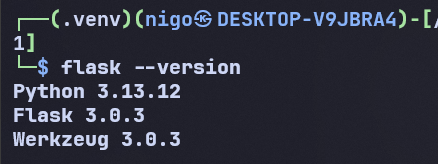
\includegraphics[width=0.9\textwidth]{pictures/flask_version.png}
  \caption{Installed tools versions verified in terminal}
\end{figure}
\textbf{git:} Installed from the official website. Configured with user name and email.
\begin{figure}[H]
  \centering
  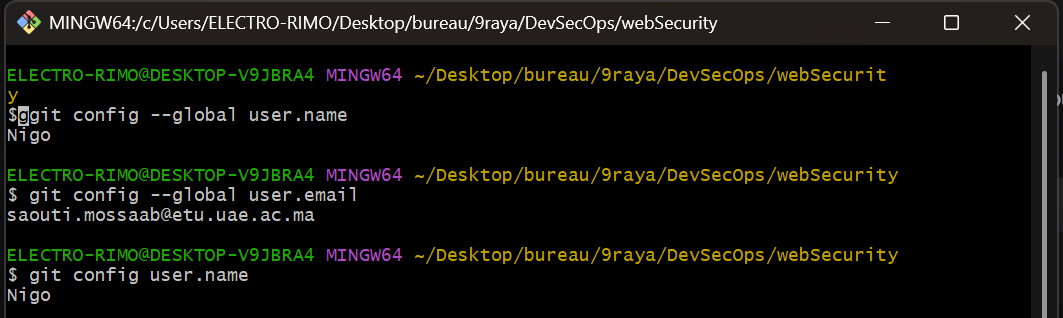
\includegraphics[width=0.9\textwidth]{pictures/git_setup.png}
  \caption{Configuration of Git in Terminal}
\end{figure}
\textbf{vscode:} Installed from the official website. \n
\textbf{postman:} Installed from the official website for API testing.
\begin{figure}[H]
  \centering
  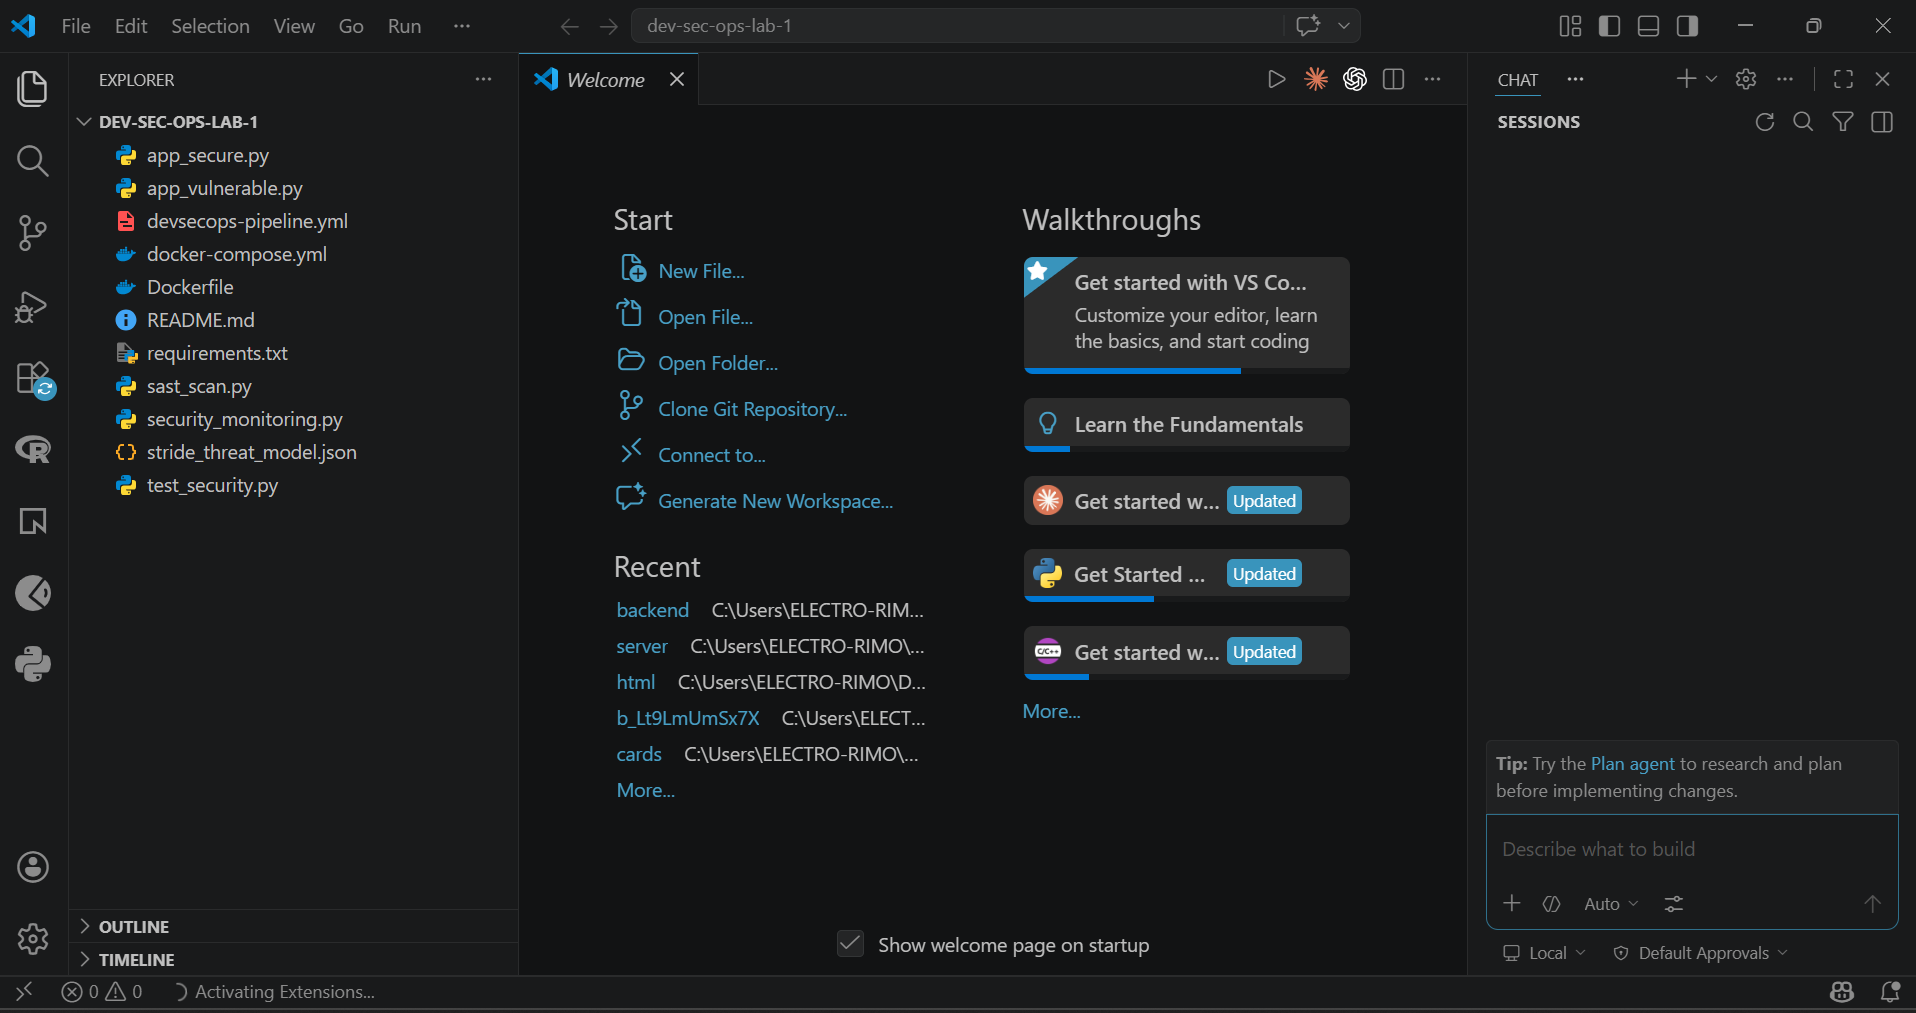
\includegraphics[width=0.45\textwidth]{pictures/vsCode.png}
  \hfill
  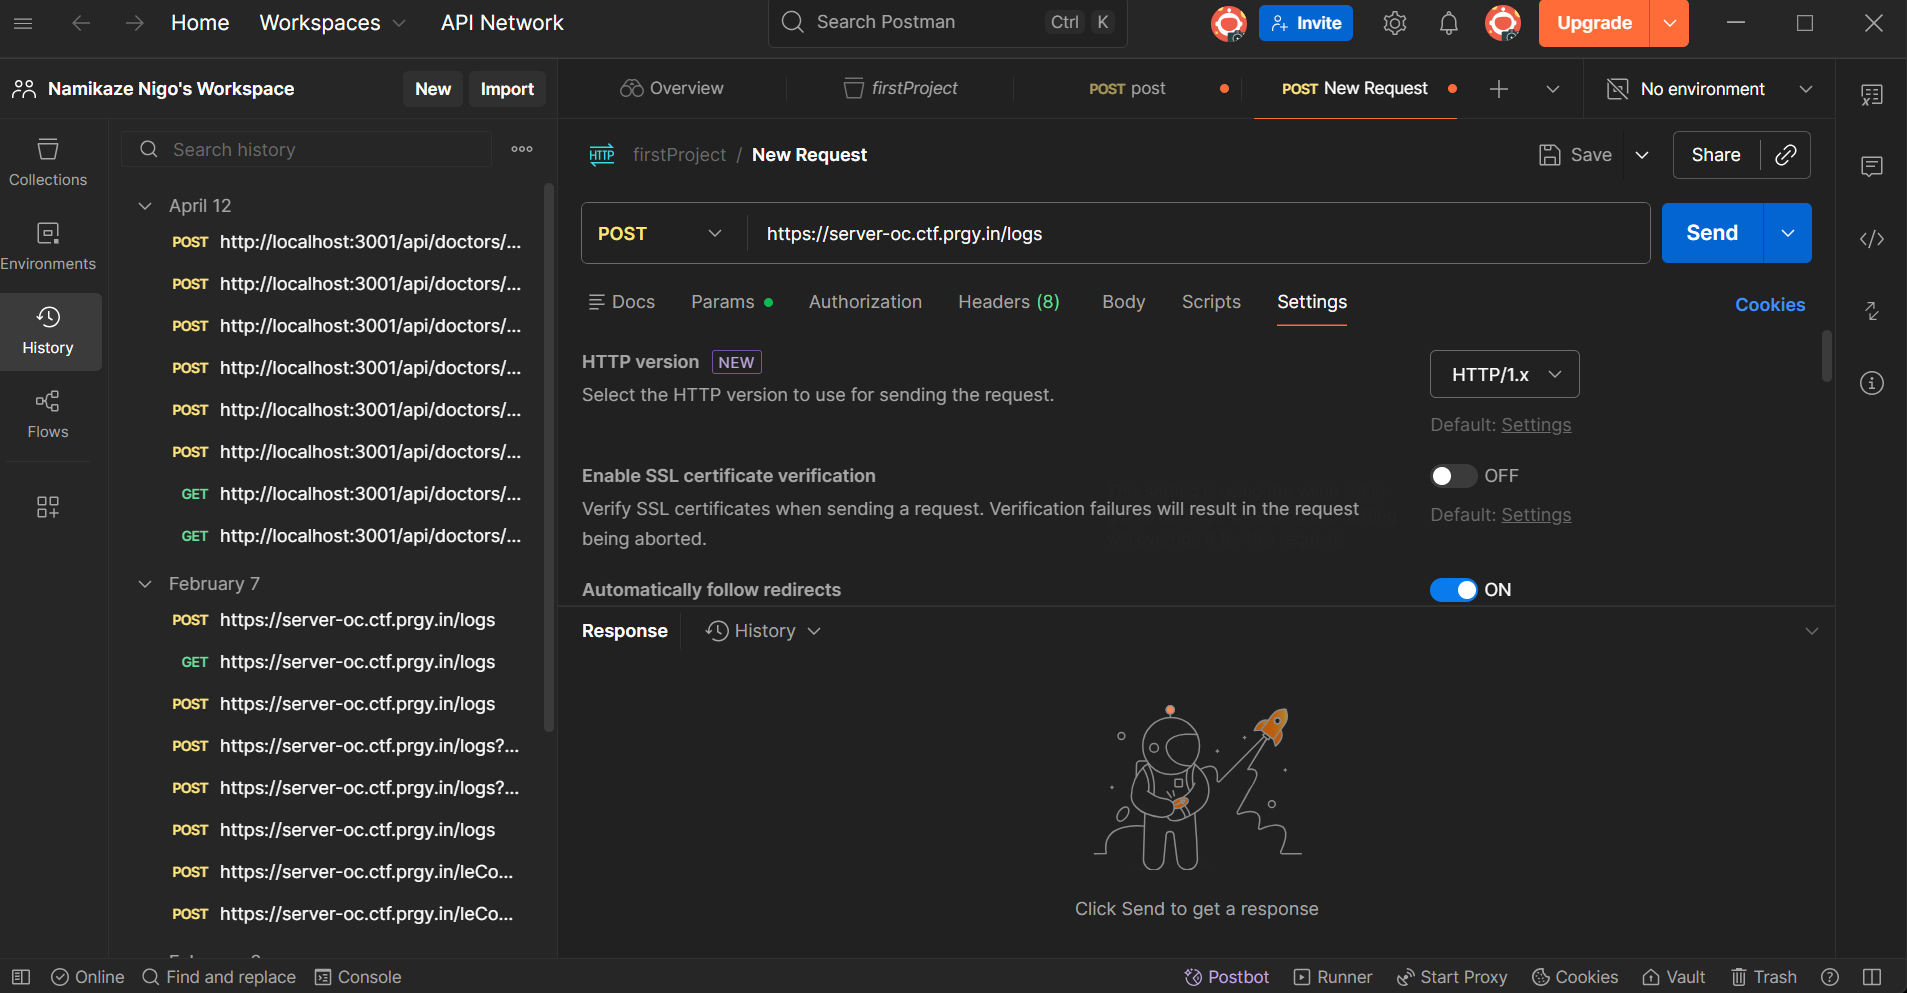
\includegraphics[width=0.45\textwidth]{pictures/postman.png}
  \caption{VS Code and Postman — development and testing environment}
\end{figure}
\textbf{Docker:} Installed from the official website. WSL integration enabled for Linux containers.
\begin{figure}[H]
  \centering
  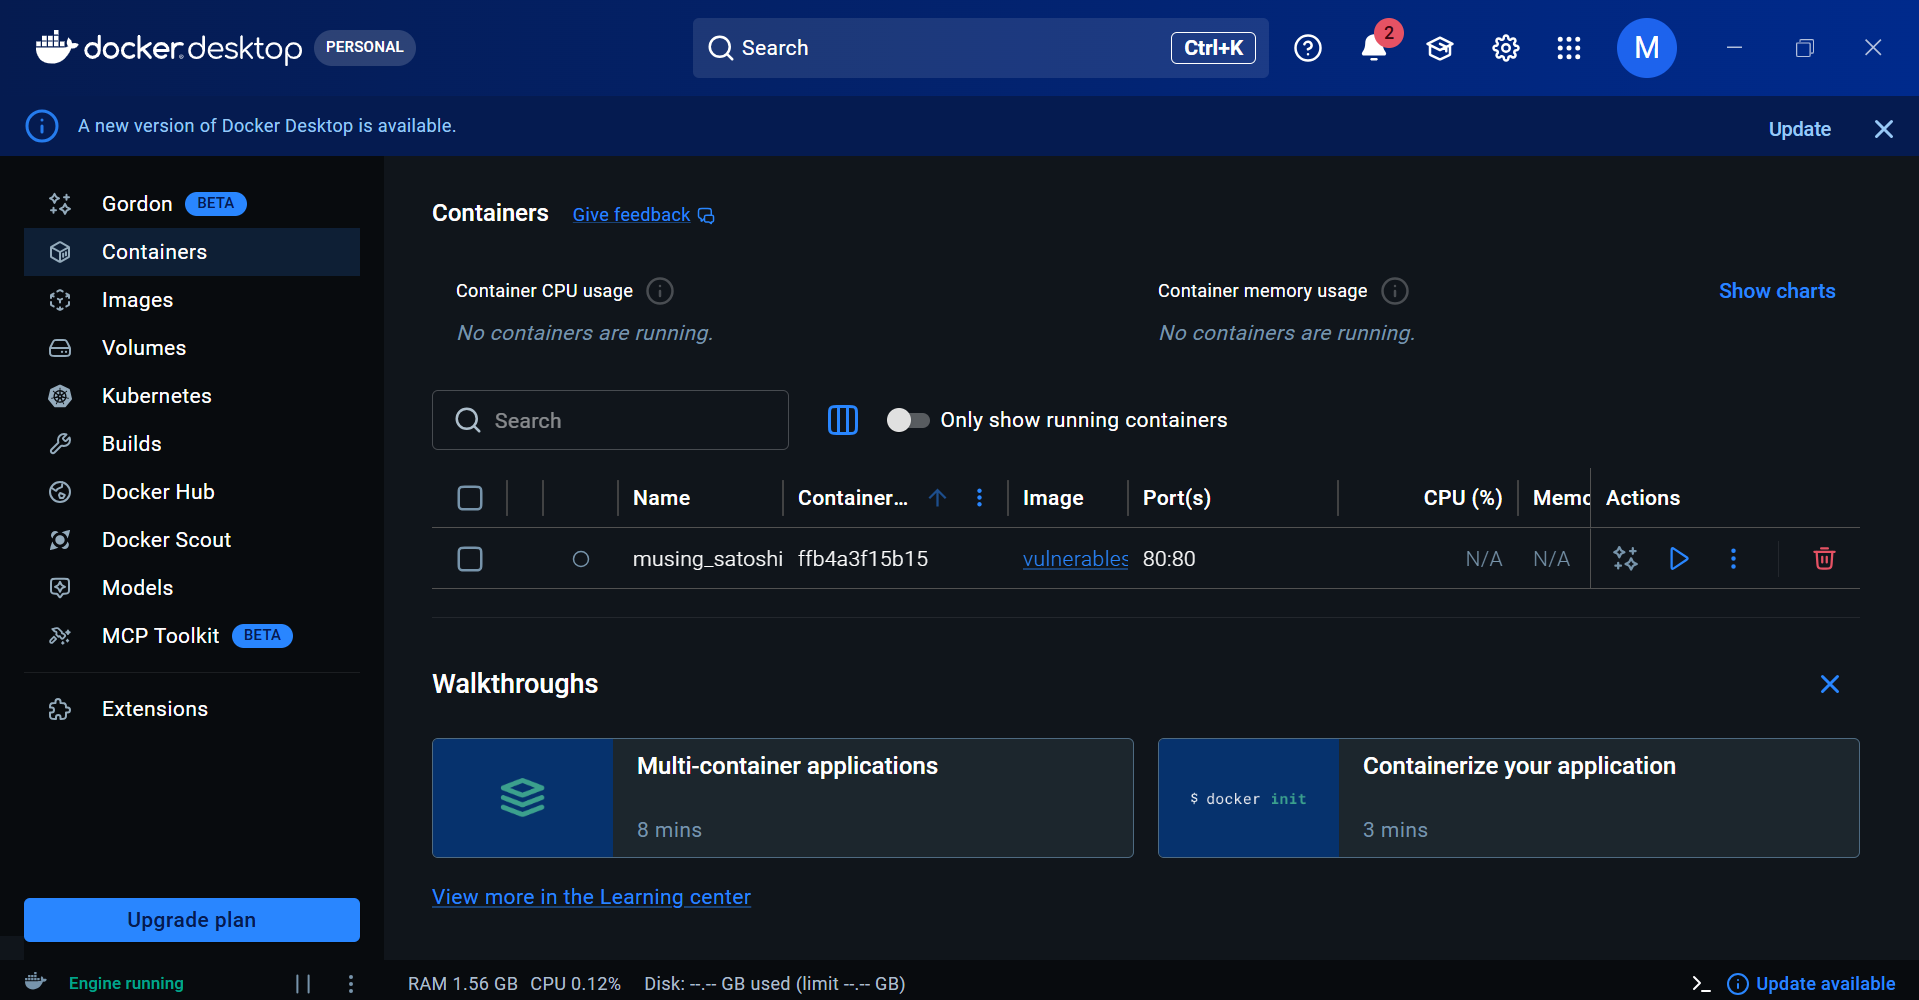
\includegraphics[width=0.9\textwidth]{pictures/docker.png}
  \caption{Docker Desktop installed}
\end{figure}



\section{Repository Setup}

The lab repository was cloned from GitHub and dependencies were installed inside a Python virtual environment to ensure isolation from the system Python installation:

\begin{lstlisting}[style=bashstyle, caption={Repository setup commands}]
git clone https://github.com/said-dev-ops/dev-sec-ops-lab-1.git
cd dev-sec-ops-lab-1
python -m venv .venv
source .venv/bin/activate   
pip install -r requirements.txt
\end{lstlisting}

% Screenshot placeholder
\begin{figure}[H]
  \centering
  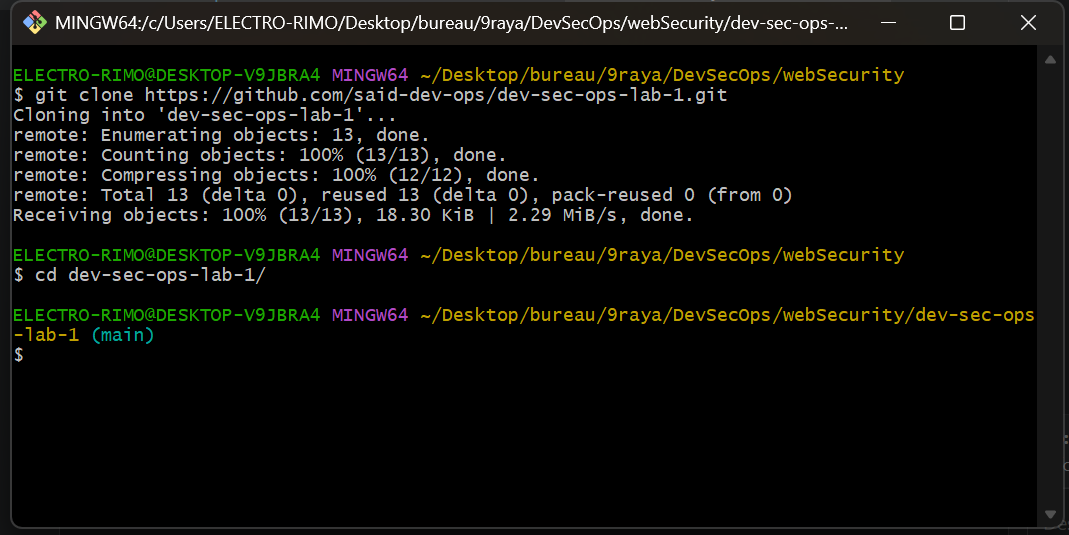
\includegraphics[width=0.45\textwidth]{pictures/cloneRepo.png}
  \hfill
  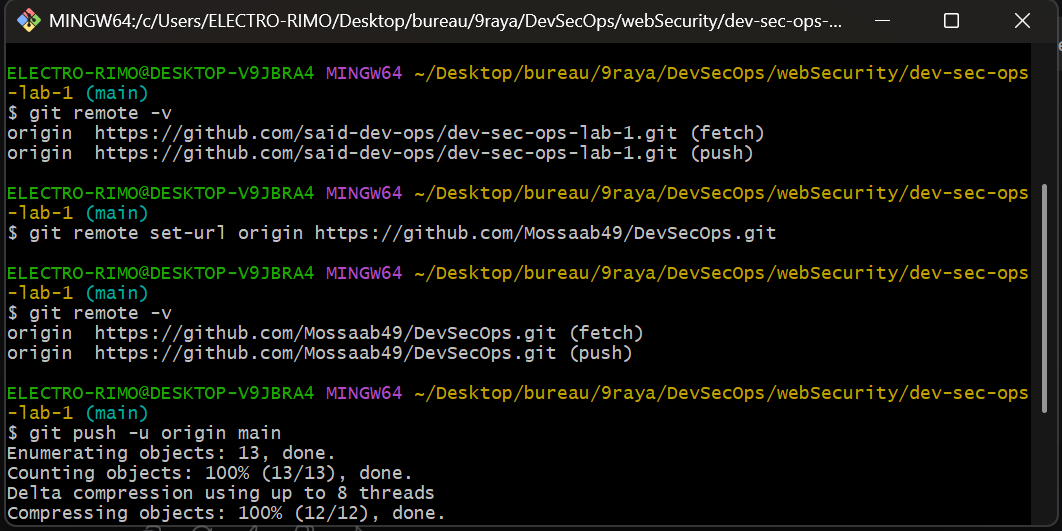
\includegraphics[width=0.45\textwidth]{pictures/change_origin.png}
  \caption{Cloning the lab repository and changing Git origin to personal fork}
\end{figure}

\begin{figure}[H]
  \centering
  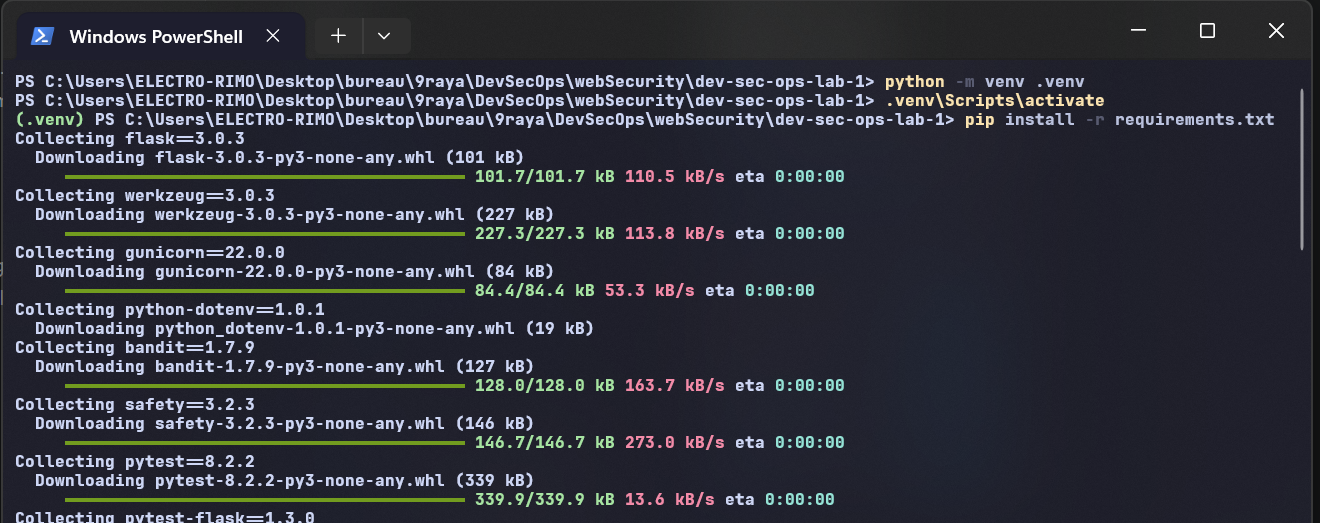
\includegraphics[width=0.9\textwidth]{pictures/setupVenv.png}
  \caption{Setting up virtual environment and installing dependencies successfully}
\end{figure}

\section{Windows vs WSL Context}

Initial setup was performed on Windows. However, the lab exercises involving Linux-specific commands (such as \texttt{cat /etc/passwd} and \texttt{ls /home}) required a Linux environment. The environment was therefore migrated to \textbf{WSL (Windows Subsystem for Linux)} running Ubuntu, which provided a realistic Linux server context while maintaining the Windows host machine. All subsequent exploitation exercises were performed inside WSL.

\begin{infobox}
\textbf{Note:} On Windows, the ping command uses \texttt{-n} instead of \texttt{-c}, and system files like \texttt{/etc/passwd} do not exist. WSL was used to replicate a realistic Linux production server environment, as intended by the lab design.
\end{infobox}

\section{Project Structure}

Following the lab instructions, the repository files were organized into three directories corresponding to the three lab parts:

\begin{lstlisting}[style=bashstyle, caption={Project directory structure}]
dev-sec-ops-lab-1/
|-- part1/
|   |-- app_vulnerable.py
|   |-- app_secure.py
|   `-- stride_threat_model.json
|-- part2/
|   |-- sast_scan.py
|   |-- test_security.py
|   `-- devsecops-pipeline.yml
`-- part3/
    |-- security_monitoring.py
    |-- Dockerfile
    `-- docker-compose.yml
\end{lstlisting}

% Screenshot placeholder
\begin{figure}[H]
  \centering
  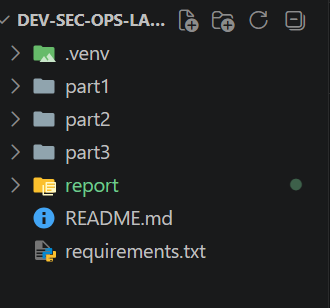
\includegraphics[width=0.9\textwidth]{pictures/tree.png}
  \caption{Organized project directory structure}
\end{figure}

% ════════════════════════════════════════════════════════════════════════════
\chapter{Threat Modeling}
% ════════════════════════════════════════════════════════════════════════════

\section{STRIDE Methodology}

Threat modeling is a structured approach to identifying security risks before writing a single line of code. \textbf{STRIDE} is a mnemonic developed by Microsoft that categorizes threats into six categories:

\begin{table}[H]
\centering
\begin{tabularx}{\textwidth}{>{\bfseries}l l l l}
\toprule
Category & Full Name & Example Threat & Control \\
\midrule
S & Spoofing & SQL injection to bypass login & Parameterized queries \\
T & Tampering & Malicious pickle deserialization & Input validation \\
R & Repudiation & No logs — cannot trace attacker & Audit logging \\
I & Info Disclosure & API returns plaintext passwords & Access control \\
D & Denial of Service & Command injection crashes server & Rate limiting, WAF \\
E & Elevation of Privilege & Path traversal reads /etc/passwd & Least privilege, safe\_join \\
\bottomrule
\end{tabularx}
\caption{STRIDE threat categories}
\end{table}

\section{Threat Modeling Process}

The threat modeling process followed these steps:

\begin{enumerate}[leftmargin=1.5cm]
  \item \textbf{Define scope} — identify assets and trust boundaries
  \item \textbf{Create a Data Flow Diagram (DFD)} — Browser $\rightarrow$ Flask $\rightarrow$ SQLite $\rightarrow$ OS
  \item \textbf{Enumerate threats} using STRIDE for each data flow
  \item \textbf{Score each threat} using DREAD or CVSS
  \item \textbf{Prioritize and assign mitigations}
  \item \textbf{Validate mitigations} and retest
\end{enumerate}

\section{Threat Register — Full Risk Assessment}

The following table maps all identified threats to STRIDE categories, attack vectors, and mitigations:

\begin{table}[H]
\centering
\begin{tabularx}{\textwidth}{>{\bfseries}l X l X l}
\toprule
ID & Threat & STRIDE & Mitigation & Status \\
\midrule
T1 & SQL Injection Login Bypass & Spoofing & Parameterized queries & \textcolor{codegreen}{\textbf{Fixed}} \\
T2 & Pickle Deserialization RCE & Tampering & Use JSON, never pickle & \textcolor{codegreen}{\textbf{Fixed}} \\
T3 & No Audit Logging & Repudiation & Log auth + admin actions & \textcolor{codegreen}{\textbf{Fixed}} \\
T4 & Password Exposure via API & Info Disclosure & Field filtering + auth & \textcolor{codegreen}{\textbf{Fixed}} \\
T5 & OS Command Injection & Denial of Service & Arg list, no shell=True & \textcolor{codegreen}{\textbf{Fixed}} \\
T6 & Path Traversal File Read & Elevation of Priv. & safe\_join + whitelist & \textcolor{codegreen}{\textbf{Fixed}} \\
T7 & Reflected XSS & Info Disclosure & Jinja2 auto-escape + CSP & \textcolor{codegreen}{\textbf{Fixed}} \\
T8 & Hardcoded Secret Key & Spoofing & Load from env variable & \textcolor{codegreen}{\textbf{Fixed}} \\
\bottomrule
\end{tabularx}
\caption{Complete threat register}
\end{table}

% Screenshot placeholder
\begin{figure}[H]
  \centering
  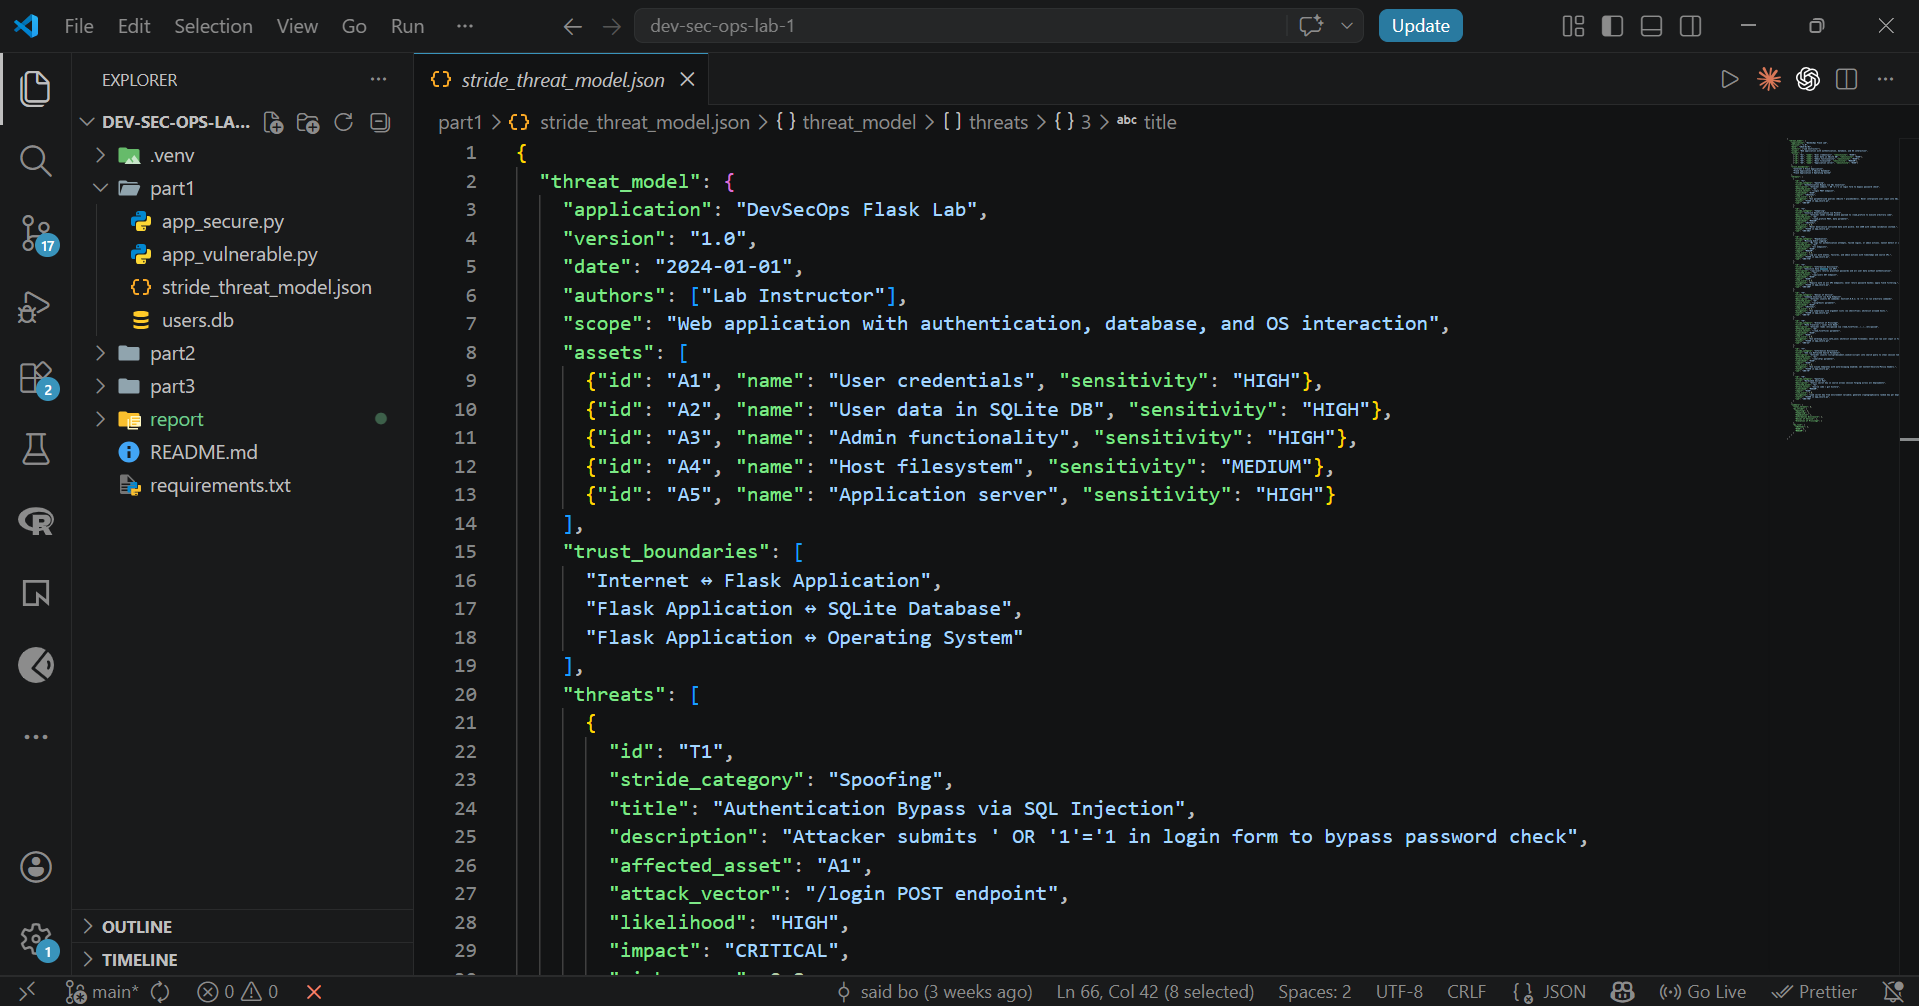
\includegraphics[width=0.9\textwidth]{pictures/threat_model.png}
  \caption{STRIDE threat model JSON file}
\end{figure}

% ════════════════════════════════════════════════════════════════════════════
\chapter{Part 1 — Build \& Break}
% ════════════════════════════════════════════════════════════════════════════

% ────────────────────────────────────────────────────────────────────────────
\section{Vulnerability Exploitation}
% ────────────────────────────────────────────────────────────────────────────

The vulnerable application was launched using:

\begin{lstlisting}[style=bashstyle]
cd part1
python app_vulnerable.py
\end{lstlisting}

% Screenshot placeholder
\begin{figure}[H]
  \centering
  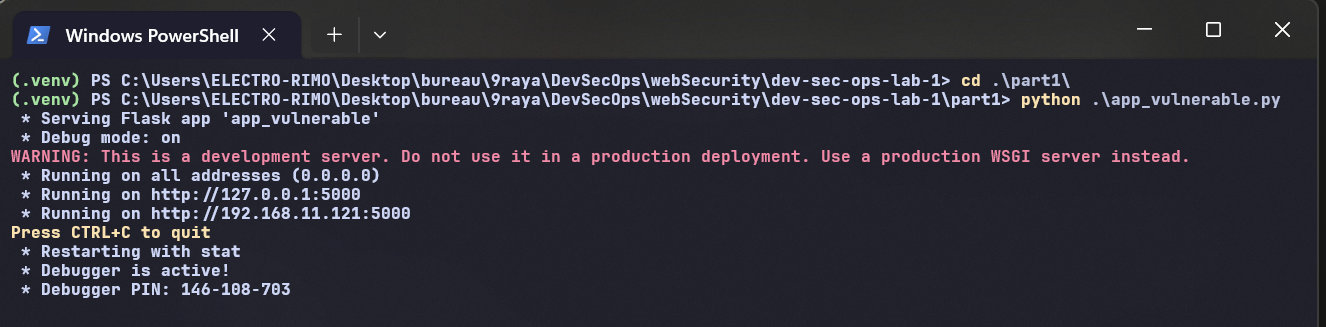
\includegraphics[width=0.45\textwidth]{pictures/run_tem.png}
  \hfill
  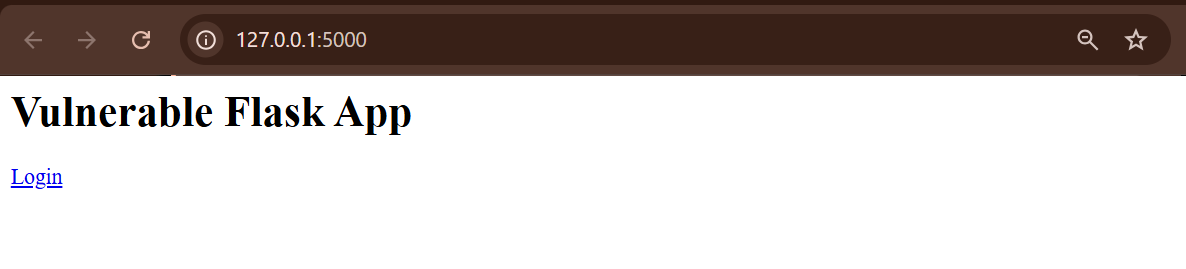
\includegraphics[width=0.45\textwidth]{pictures/run_brows.png}
  \caption{Vulnerable Flask application running}
\end{figure}

% ────────────────────────────────────────────────────────────────────────────
\subsection{Exercise 1 — SQL Injection (T1)}
% ────────────────────────────────────────────────────────────────────────────

\textbf{Attack Description}

SQL Injection occurs when user-supplied input is directly concatenated into an SQL query without sanitization. An attacker can manipulate the query logic to bypass authentication, extract data, or modify the database.

\textbf{Target:} \texttt{POST /login}

\textbf{Exploitation}

The following payload was entered in the username field on the login page:

\begin{lstlisting}[style=urlstyle, caption={SQL Injection payload}]
admin' OR '1'='1
\end{lstlisting}

The injected query becomes:
\begin{lstlisting}[style=pythonstyle, caption={Resulting malicious SQL query}]
SELECT * FROM users WHERE username='admin' OR '1'='1'
\end{lstlisting}

Since \texttt{'1'='1'} is always true, the query returns the admin creedentials, completely bypassing authentication.

% Screenshot placeholders
\begin{figure}[H]
  \centering
    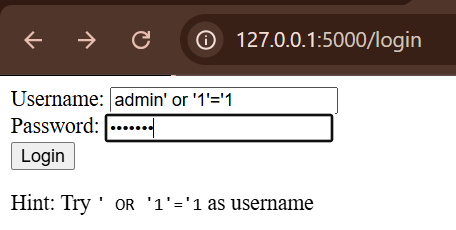
\includegraphics[width=0.45\textwidth]{pictures/login.png}
  \caption{Login page — target of SQL injection attack}
\end{figure}

\begin{figure}[H]
  \centering
    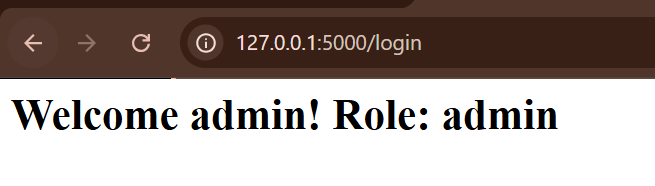
\includegraphics[width=0.45\textwidth]{pictures/dashboard.png}
  \caption{Authentication bypassed using SQL injection}
\end{figure}

\textbf{Impact Analysis}

\begin{warningbox}
\textbf{STRIDE Category:} Spoofing (T1) \\
\textbf{CVSS Score:} 9.8 Critical \\
\textbf{Impact:} An attacker can authenticate as any user, including administrators, without knowing any password. This grants full unauthorized access to the application.
\end{warningbox}

% ────────────────────────────────────────────────────────────────────────────
\subsection{Exercise 2 — Cross-Site Scripting (XSS) (T7)}
% ────────────────────────────────────────────────────────────────────────────

\textbf{Attack Description}

Reflected XSS occurs when user input is included in the HTTP response without proper escaping. An attacker can inject malicious JavaScript that executes in the victim's browser, potentially stealing session tokens or performing actions on their behalf.

\textbf{Target:} \texttt{GET /search?q=}

\textbf{Exploitation}

The following payloads were tested:

\begin{lstlisting}[style=urlstyle, caption={XSS Payload 1 — script tag}]
http://127.0.0.1:5000/search?q=<script>alert(document.cookie)</script>
\end{lstlisting}

\begin{lstlisting}[style=urlstyle, caption={XSS Payload 2 — image error event}]
http://127.0.0.1:5000/search?q=<img src=x onerror=alert(1)>
\end{lstlisting}

Both payloads triggered a JavaScript alert in the browser. The \texttt{document.cookie} payload returned an empty value because Flask sets the \texttt{HttpOnly} flag on session cookies, preventing JavaScript access. However, the XSS vulnerability itself was confirmed — in a real scenario targeting an application without \texttt{HttpOnly}, session tokens would be exfiltrated.

% Screenshot placeholders
\begin{figure}[H]
  \centering
  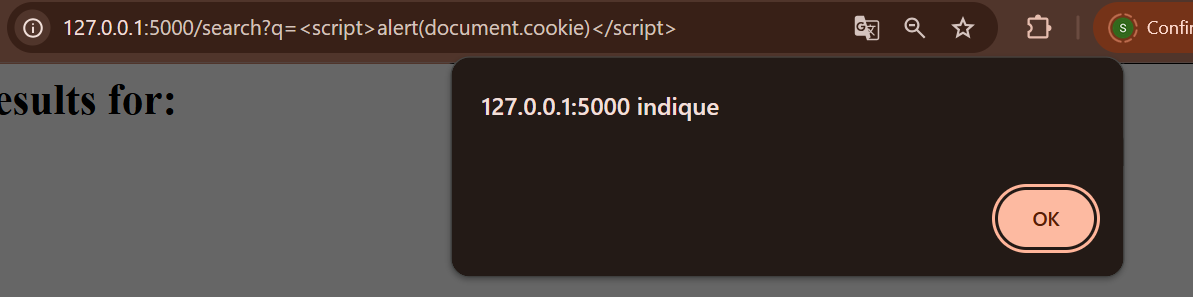
\includegraphics[width=0.45\textwidth]{pictures/xss_cookies.png}
  \caption{XSS payload executing JavaScript alert in browser}
\end{figure}

\begin{figure}[H]
  \centering
    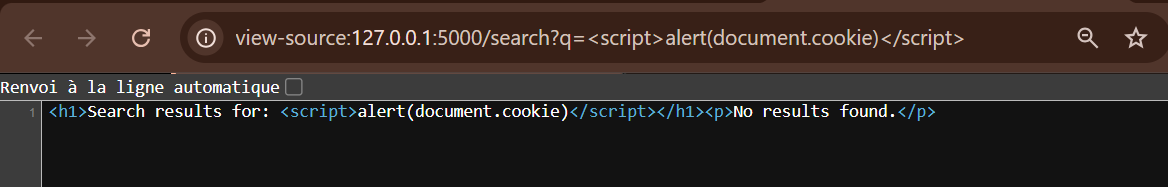
\includegraphics[width=0.45\textwidth]{pictures/xss_source.png}
  \caption{Page source confirming lack of output encoding}
\end{figure}

\textbf{Impact Analysis}

\begin{warningbox}
\textbf{STRIDE Category:} Information Disclosure (T7) \\
\textbf{CVSS Score:} 6.1 Medium \\
\textbf{Impact:} An attacker can craft a malicious URL and send it to victims. When clicked, the script executes in the victim's browser and can steal cookies, redirect to phishing pages, or perform actions on behalf of the user.
\end{warningbox}

% ────────────────────────────────────────────────────────────────────────────
\subsection{Exercise 3 — OS Command Injection (T5)}
% ────────────────────────────────────────────────────────────────────────────

\textbf{Attack Description}

Command injection occurs when user input is passed unsanitized to a system shell command. Using \texttt{shell=True} in Python's \texttt{subprocess} module passes the entire string directly to the OS shell, allowing an attacker to append additional commands using shell operators.

\textbf{Target:} \texttt{GET /ping?host=}

\textbf{Windows vs WSL Context}

Initial testing was performed on Windows where Linux-specific commands were unavailable. The \texttt{ping} command on Windows uses \texttt{-n} instead of \texttt{-c}, and system files like \texttt{/etc/passwd} do not exist. The environment was migrated to WSL to replicate a realistic Linux server scenario.

On Windows, the pipe operator (\texttt{|}) was used to confirm command injection:

\begin{lstlisting}[style=urlstyle, caption={Windows command injection — whoami}]
http://127.0.0.1:5000/ping?host=127.0.0.1|whoami
\end{lstlisting}

The server returned: \texttt{desktop-v9jbra4\textbackslash electro-rimo}, confirming arbitrary command execution.

After migrating to WSL, Linux commands worked as intended:

\begin{lstlisting}[style=urlstyle, caption={WSL command injection — list home directory}]
http://127.0.0.1:5000/ping?host=127.0.0.1;ls+/home
\end{lstlisting}

\begin{lstlisting}[style=urlstyle, caption={WSL command injection — dump system users}]
http://127.0.0.1:5000/ping?host=127.0.0.1;cat+/etc/passwd
\end{lstlisting}

% Screenshot placeholders
\begin{figure}[H]
  \centering
    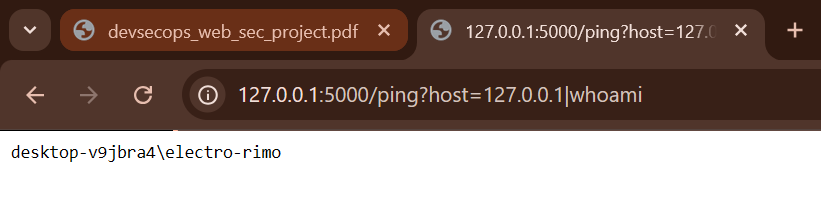
\includegraphics[width=0.45\textwidth]{pictures/whoami_wind.png}
  \caption{Command injection confirmed on Windows — whoami executed}
\end{figure}

\begin{figure}[H]
  \centering
  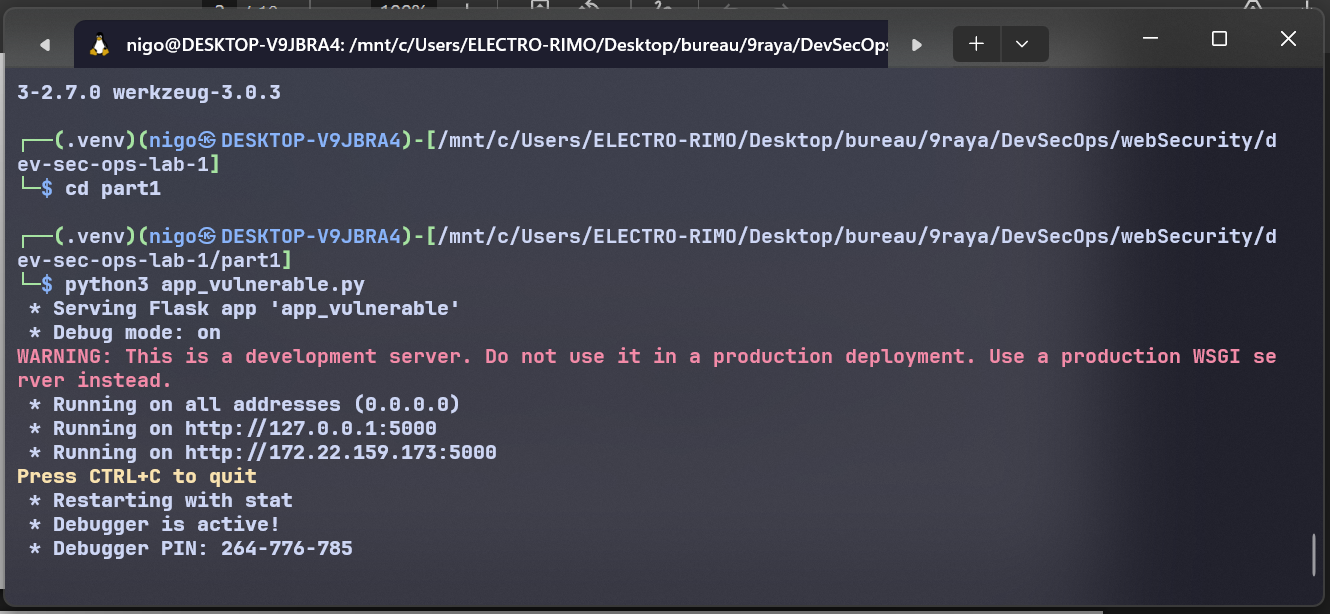
\includegraphics[width=0.45\textwidth]{pictures/setup_env_wsl.png}
  \hfill
  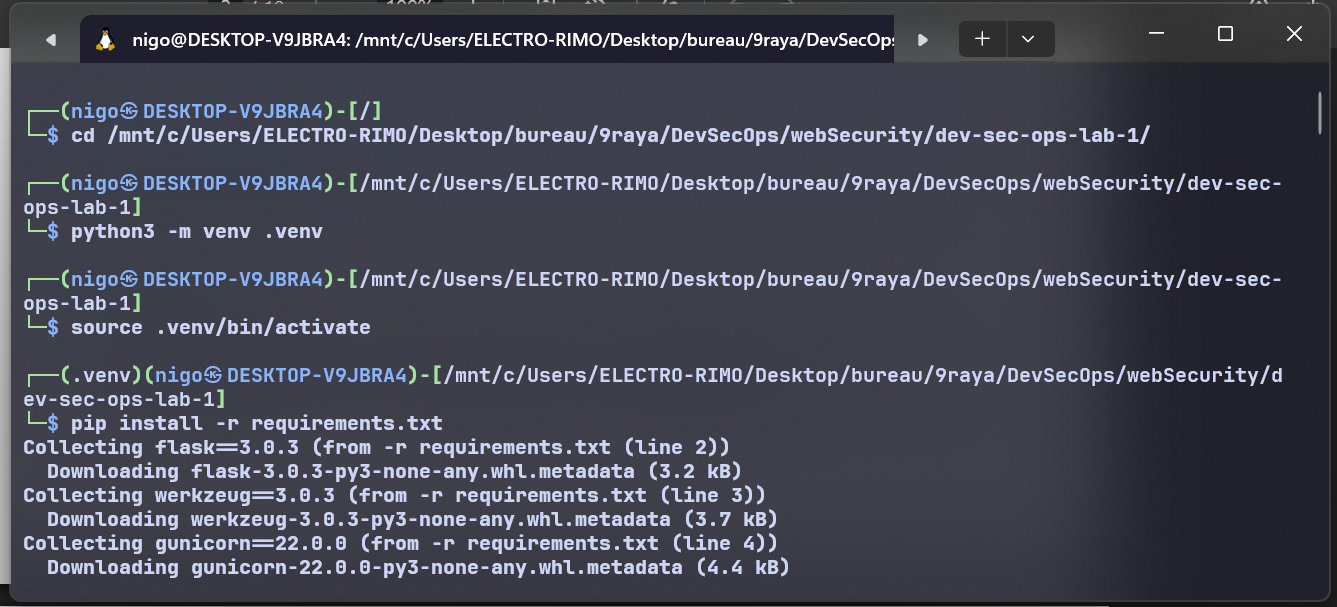
\includegraphics[width=0.45\textwidth]{pictures/run_wsl.png}
  \caption{setup and run vulnerable app in WSL for Linux command testing}
\end{figure}

\begin{figure}[H]
  \centering
    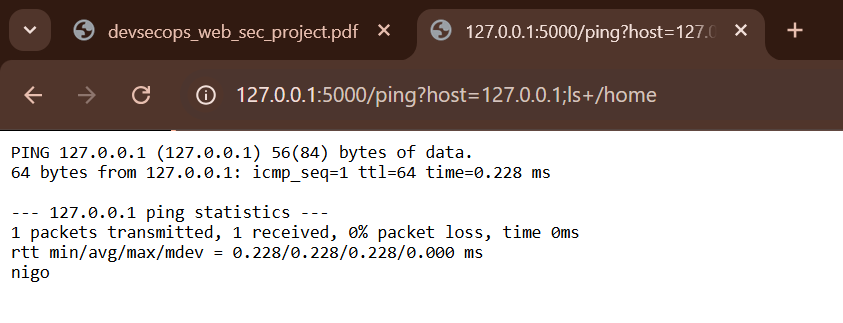
\includegraphics[width=0.45\textwidth]{pictures/ls_wsl.png}
  \caption{Home directory listing via command injection on WSL}
\end{figure}

\begin{figure}[H]
  \centering
    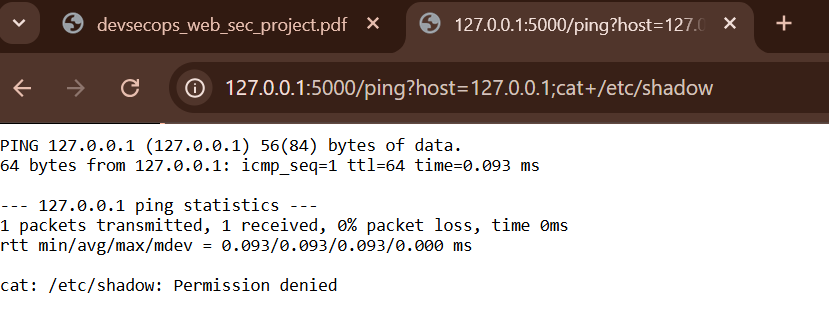
\includegraphics[width=0.45\textwidth]{pictures/cat_passwd.png}
  \caption{System user file exposed via command injection}
\end{figure}

\textbf{Impact Analysis}

\begin{warningbox}
\textbf{STRIDE Category:} Denial of Service / Elevation of Privilege (T5) \\
\textbf{CVSS Score:} 9.8 Critical \\
\textbf{Impact:} An attacker gains the ability to execute arbitrary OS commands on the server. This can lead to full system compromise: reading sensitive files, creating backdoors, exfiltrating data, or crashing the server entirely.
\end{warningbox}

% ────────────────────────────────────────────────────────────────────────────
\subsection{Exercise 4 — Path Traversal (T6)}
% ────────────────────────────────────────────────────────────────────────────

\textbf{Attack Description}

Path traversal occurs when user-supplied filenames are passed directly to file system operations without validation. Using \texttt{../} sequences, an attacker can escape the intended directory and access arbitrary files on the server.

\textbf{Target:} \texttt{GET /read\_file?file=}

\textbf{Exploitation}

\begin{lstlisting}[style=urlstyle, caption={Path traversal — read system users}]
http://127.0.0.1:5000/read_file?file=../../etc/passwd
\end{lstlisting}

\begin{lstlisting}[style=urlstyle, caption={Path traversal — read application source code}]
http://127.0.0.1:5000/read_file?file=../app_vulnerable.py
\end{lstlisting}

Both requests returned the full file contents in the browser. Notably, absolute paths also worked because the vulnerable app uses Python's raw \texttt{open()} function:

\begin{lstlisting}[style=urlstyle, caption={Absolute path attack}]
http://127.0.0.1:5000/read_file?file=/etc/passwd
\end{lstlisting}

% Screenshot placeholders
\begin{figure}[H]
  \centering
    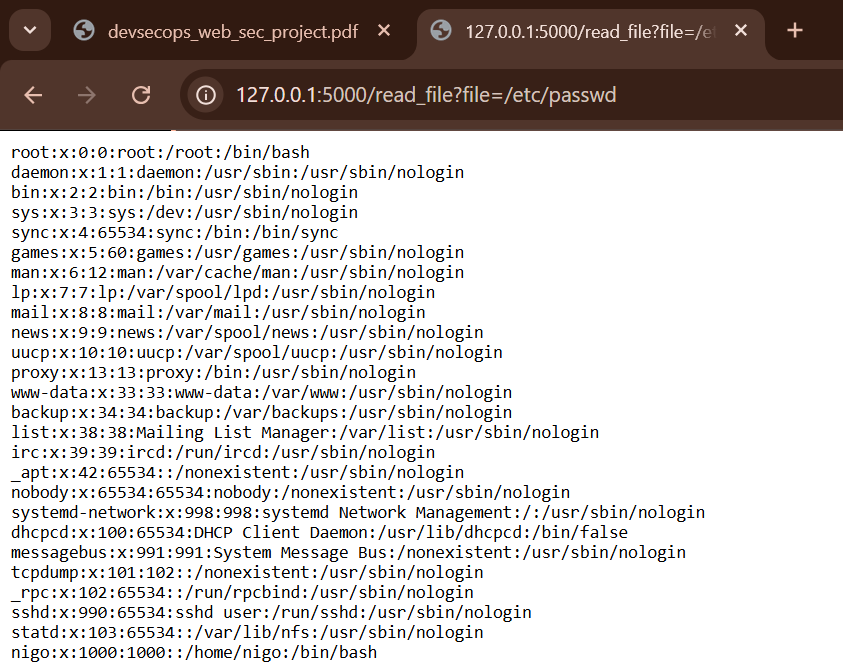
\includegraphics[width=0.45\textwidth]{pictures/file_etc.png}
  \caption{System file exposed via path traversal}
\end{figure}

\begin{figure}[H]
  \centering
    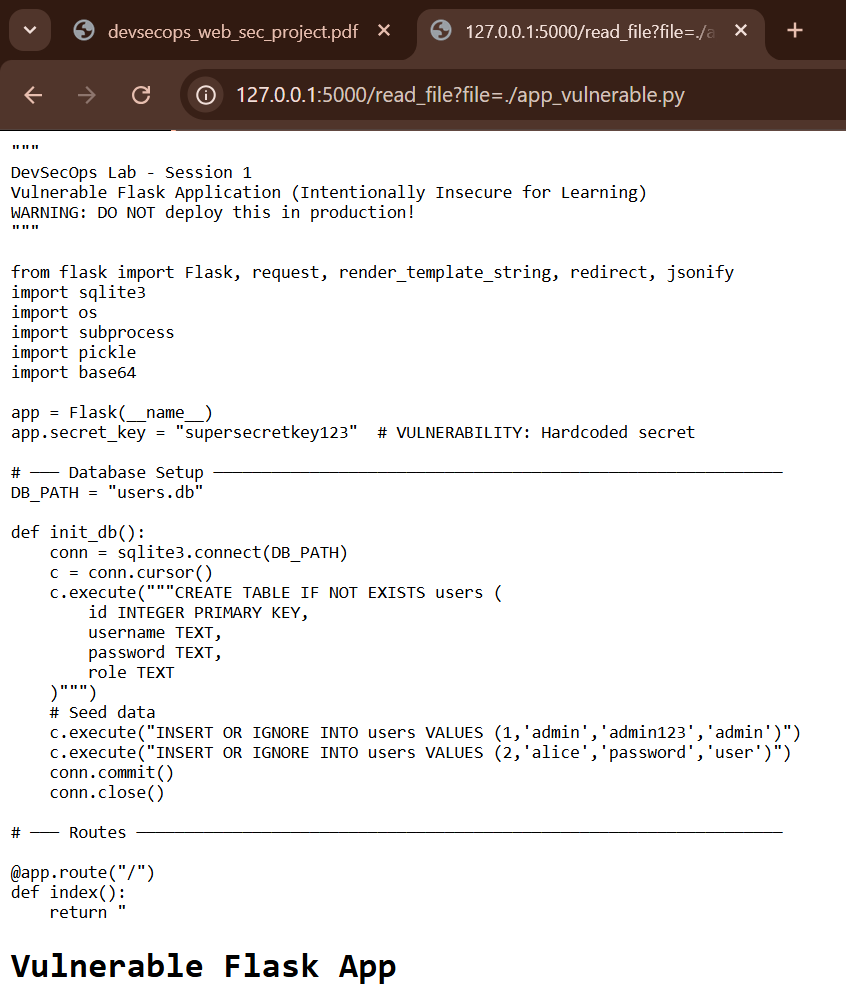
\includegraphics[width=0.45\textwidth]{pictures/app_vuln.png}
  \caption{Application source code exposed via path traversal}
\end{figure}

\textbf{Impact Analysis}

\begin{warningbox}
\textbf{STRIDE Category:} Elevation of Privilege (T6) \\
\textbf{CVSS Score:} 7.5 High \\
\textbf{Impact:} An attacker can read any file the application has permission to access, including configuration files, secret keys, SSL certificates, and the application source code itself. This information can be used to plan further attacks.
\end{warningbox}

% ════════════════════════════════════════════════════════════════════════════
\section{Secure Implementation}
% ════════════════════════════════════════════════════════════════════════════

After exploiting all vulnerabilities, \texttt{app\_secure.py} was examined to understand how each issue was remediated. The secure version follows a consistent principle: \textbf{never trust user input}.

\begin{table}[H]
\centering
\begin{tabularx}{\textwidth}{l X X}
\toprule
\textbf{\#} & \textbf{Vulnerability} & \textbf{Fix Applied} \\
\midrule
1 & SQL Injection & Parameterized queries using \texttt{?} placeholders \\
2 & XSS & Jinja2 templates with auto-escaping via \texttt{render\_template()} \\
3 & Command Injection & Subprocess list syntax + host whitelist; \texttt{shell=False} \\
4 & Path Traversal & \texttt{werkzeug.safe\_join()} + allowed filename whitelist \\
5 & Insecure Deserialization & Replace \texttt{pickle} with \texttt{json.get\_json()} + field whitelist \\
6 & Data Exposure & Remove passwords from API; require auth on all routes \\
7 & Hardcoded Secret & \texttt{os.environ.get('SECRET\_KEY')} or \texttt{secrets.token\_hex(32)} \\
8 & Debug Mode & \texttt{app.run(debug=False)}; use Gunicorn in production \\
\bottomrule
\end{tabularx}
\caption{Vulnerability fixes comparison}
\end{table}

\textbf{SQL Injection Fix:}
\begin{lstlisting}[style=pythonstyle, caption={Vulnerable vs Secure SQL query}]
# VULNERABLE
query = f"SELECT * FROM users WHERE username='{username}'"
conn.execute(query)

# SECURE
conn.execute("SELECT * FROM users WHERE username=?", (username,))
\end{lstlisting}

\textbf{Command Injection Fix:}
\begin{lstlisting}[style=pythonstyle, caption={Vulnerable vs Secure subprocess call}]
# VULNERABLE
output = subprocess.check_output(f"ping -c 1 {host}", shell=True)

# SECURE
ALLOWED_HOSTS = ["127.0.0.1", "localhost"]
if host not in ALLOWED_HOSTS:
    abort(403)
subprocess.check_output(["ping", "-c", "1", host])
\end{lstlisting}

\textbf{Path Traversal Fix:}
\begin{lstlisting}[style=pythonstyle, caption={Vulnerable vs Secure file access}]
# VULNERABLE
with open(filename) as f:
    return f.read()

# SECURE
ALLOWED_FILES = ["report.txt", "readme.txt"]
if filename not in ALLOWED_FILES:
    abort(403)
filepath = safe_join(BASE_DIR, filename)
with open(filepath) as f:
    return f.read()
\end{lstlisting}

% Screenshot placeholder
\begin{figure}[H]
  \centering
    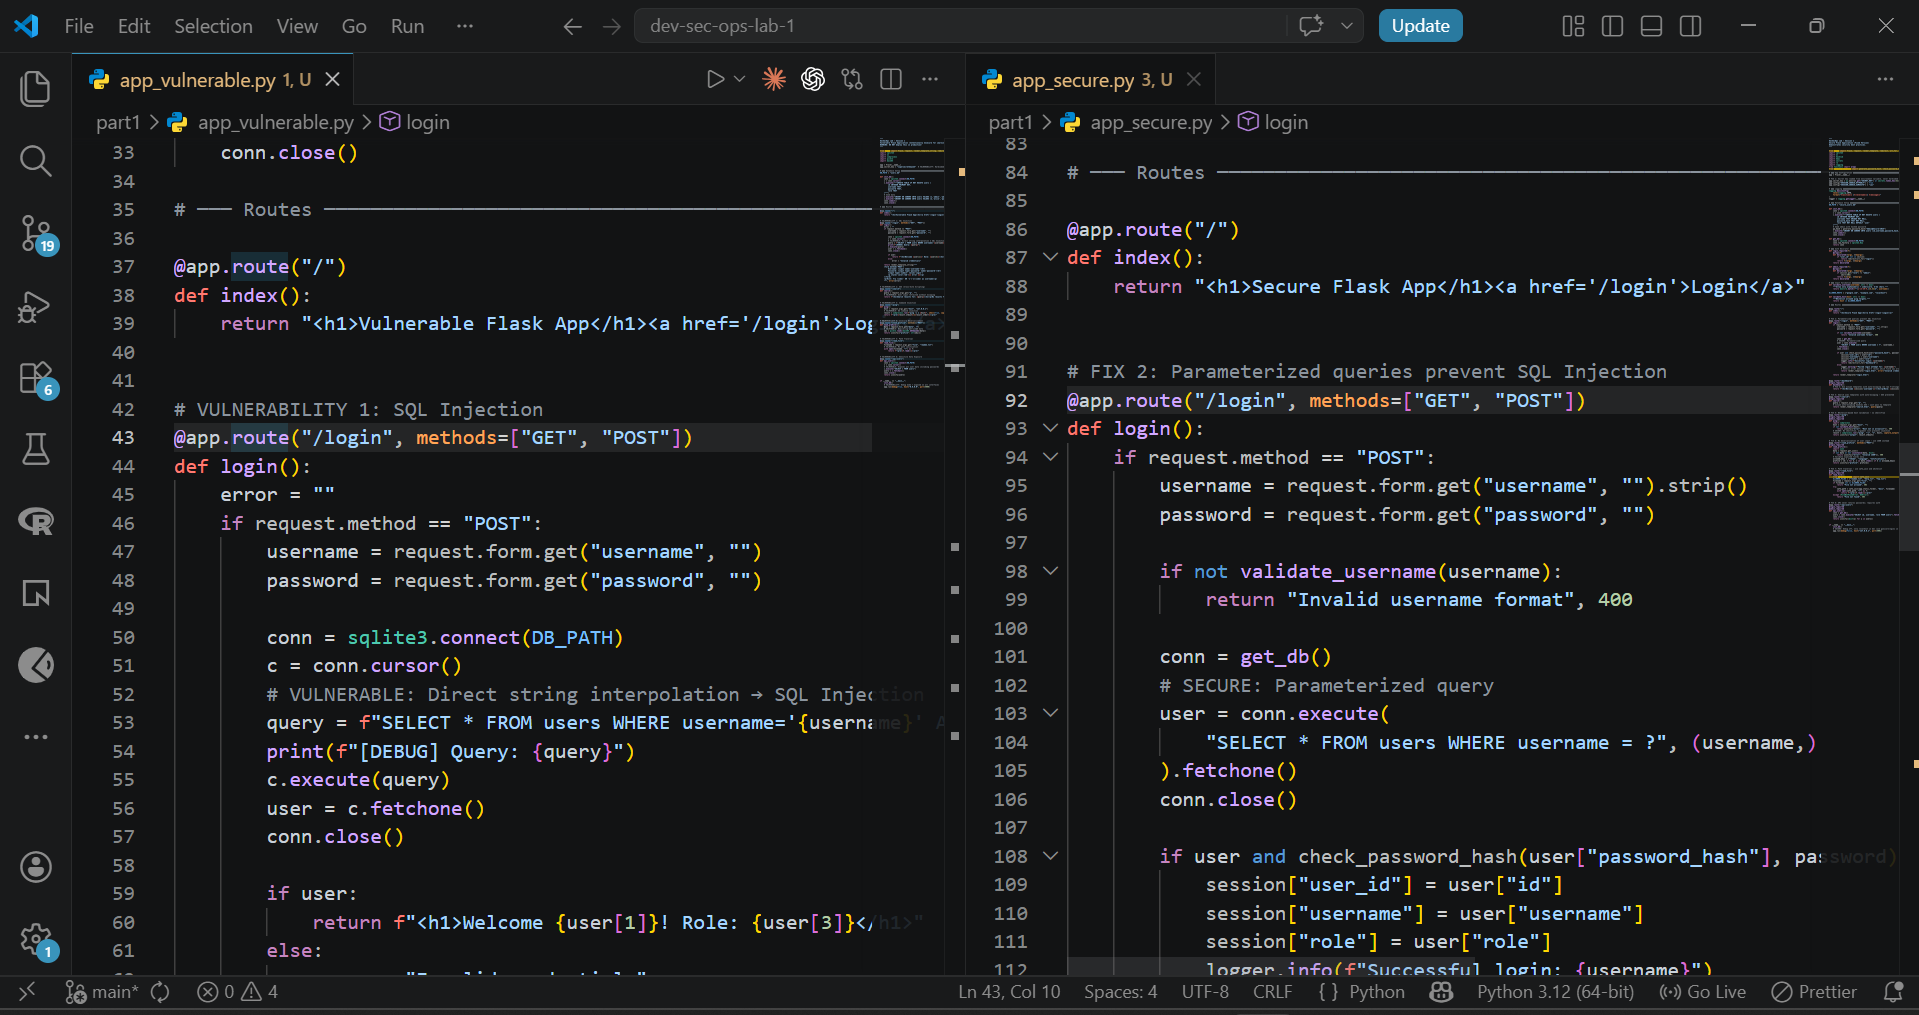
\includegraphics[width=0.45\textwidth]{pictures/app_comparison.png}
  \caption{Side-by-side comparison of vulnerable and secure implementations}
\end{figure}

\textbf{Note on \texttt{safe\_join()} behavior:}

\texttt{werkzeug.safe\_join()} blocks both relative traversal (\texttt{../}) and absolute paths (\texttt{/etc/passwd}). The following table summarizes its behavior:

\begin{table}[H]
\centering
\begin{tabular}{l c c}
\toprule
\textbf{Payload} & \textbf{Vulnerable (open())} & \textbf{Secure (safe\_join())} \\
\midrule
\texttt{../../etc/passwd} & \textcolor{accentred}{\textbf{Works}} & \textcolor{codegreen}{\textbf{Blocked}} \\
\texttt{/etc/passwd} & \textcolor{accentred}{\textbf{Works}} & \textcolor{codegreen}{\textbf{Blocked}} \\
\texttt{../app\_vulnerable.py} & \textcolor{accentred}{\textbf{Works}} & \textcolor{codegreen}{\textbf{Blocked}} \\
\texttt{report.txt} (whitelisted) & \textcolor{accentred}{\textbf{Works}} & \textcolor{codegreen}{\textbf{Allowed}} \\
\bottomrule
\end{tabular}
\caption{safe\_join() behavior against different payloads}
\end{table}

% ════════════════════════════════════════════════════════════════════════════
\chapter{Part 2 — Test \& Automate}
% ════════════════════════════════════════════════════════════════════════════

\begin{infobox}
\textbf{Note:} This chapter will be completed after finishing Part 2 of the lab. Sections covered: SAST with Bandit, SCA with Safety, Security Unit Testing with pytest, and CI/CD Pipeline with GitHub Actions.
\end{infobox}

\section{SAST — Static Application Security Testing}
% Content to be added after completing Part 2

\section{SCA — Software Composition Analysis}
% Content to be added after completing Part 2

\section{Security Unit Testing}
% Content to be added after completing Part 2

\section{CI/CD Pipeline with Security Gates}
% Content to be added after completing Part 2

% ════════════════════════════════════════════════════════════════════════════
\chapter{Part 3 — Harden \& Monitor}
% ════════════════════════════════════════════════════════════════════════════

\begin{infobox}
\textbf{Note:} This chapter will be completed after finishing Part 3 of the lab. Sections covered: Docker hardening, WAF, security headers, and incident response.
\end{infobox}

\section{Docker Security Hardening}
% Content to be added after completing Part 3

\section{Runtime Security Monitoring}
% Content to be added after completing Part 3

\section{Security Headers}
% Content to be added after completing Part 3

\section{Incident Response Exercise}
% Content to be added after completing Part 3

% ════════════════════════════════════════════════════════════════════════════
\chapter{Conclusion}
% ════════════════════════════════════════════════════════════════════════════

\begin{infobox}
\textbf{Note:} Conclusion to be written after completing all three parts of the lab.
\end{infobox}

% ════════════════════════════════════════════════════════════════════════════
\chapter*{References}
\addcontentsline{toc}{chapter}{References}
% ════════════════════════════════════════════════════════════════════════════

\begin{enumerate}
  \item OWASP Top Ten. \textit{OWASP Foundation}. \url{https://owasp.org/www-project-top-ten/}
  \item STRIDE Threat Modeling. \textit{Microsoft Security}. \url{https://learn.microsoft.com/en-us/azure/security/develop/threat-modeling-tool-threats}
  \item Bandit Documentation. \textit{PyCQA}. \url{https://bandit.readthedocs.io/}
  \item Safety Documentation. \url{https://pyup.io/safety/}
  \item CIS Docker Benchmark v1.6. \textit{Center for Internet Security}.
  \item Werkzeug Documentation — safe\_join. \url{https://werkzeug.palletsprojects.com/}
  \item Flask Security Documentation. \url{https://flask.palletsprojects.com/en/latest/security/}
  \item Lab Repository. \url{https://github.com/said-dev-ops/dev-sec-ops-lab-1}
\end{enumerate}

\end{document}
